\chapter{研究背景}
\label{chap:background}

本章では、本研究が取り扱うリアルタイム情報共有するシステムの現在の状況や情報表現の工夫について述べる。

\newpage

\section{タイムライン表示}

チャット(図\ref{chat})はインターネットを利用したテキストベースのリアルタイムコミュニケーションシステムである。
かつてはテキストを介して参加者がコミュニケーションを取るだけであったが、
現在はテキストだけでなく画像や音声などもやりとりすることができる。
チャットは数文字〜数十文字程度の文章を書き込んでやりとりすることがほとんどだが、
文字入力が間に合わず話題についていくことができなくなってしまうことがあるため、
「>」(特定の相手に対する発言)や「/」(発言の区切り)などといった記号による簡略的な表現や、
「ALL」(全員)や「ROM」(Read Only Member)などといった略語を用いて会話を行うことが多い。

また、多くのチャットのインタフェースは参加者の投稿を表示する時系列に表示するタイムライン表示を利用している。
タイムライン表示はTwitter、FacebookなどのSNSのリアルタイムのコミュニケーションや
天気予報(図\ref{weather})、株価など時間で推移する情報の表示に現在最も普及している視覚化手法である。

\begin{figure}[H]
\centering
\fbox{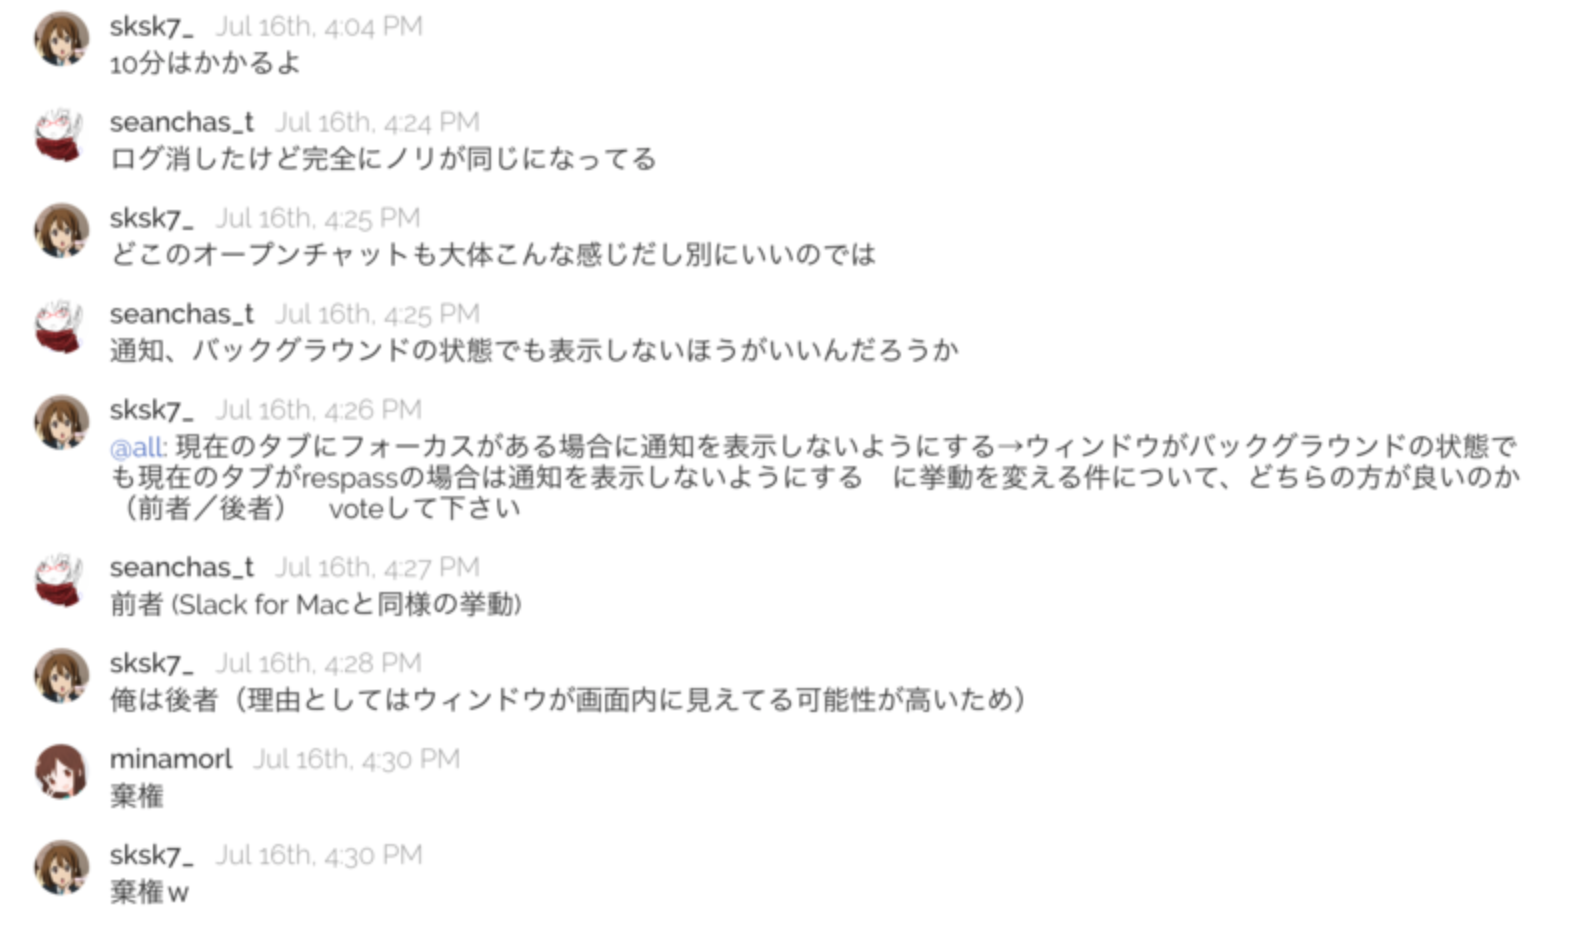
\includegraphics[width=9cm]{images/chat.png}}
\caption{一般的なテキストチャット}
\label{chat}
\end{figure}

\begin{figure}[H]
\centering
\fbox{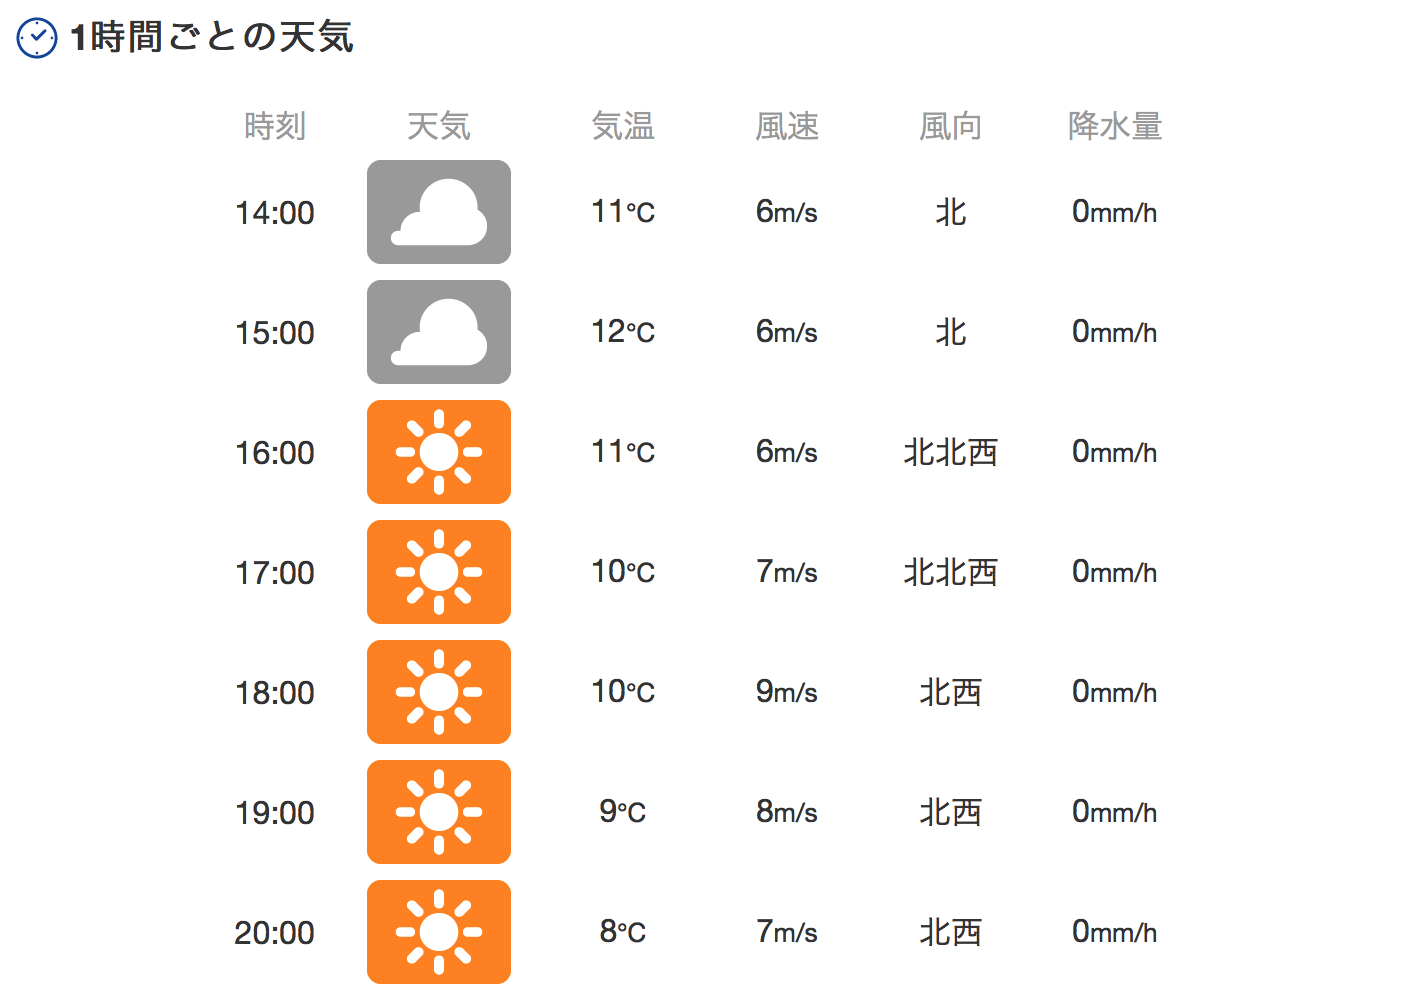
\includegraphics[width=9cm]{images/weather.png}}
\caption{時系列順に表示される天気予報}
\label{weather}
\end{figure}

日本の若者を中心に人気のコミュニケーションサービスLINE\footnote{\textsf{https://line.me/ja/}}
のトーク機能では、
テキストとは別に{\bf スタンプ}と呼ばれる大型のピクトグラムを相手に送ることができるのが特徴である。
スタンプはタイムライン表示の中で情報を目立たせたい時に使用され、
テキストで記述するのが難しい表現や感情を伝えたり,
テキストを考えて入力するよりも速くて簡単であったりすることから、
非常に便利なコミュニケーションとして浸透しつつある。
LINEは日本の20代の92.2\%が利用しているという圧倒的なシェアを誇っており\cite{soumu27}、
スタンプによるコミュニケーションもまた多くの人に利用されている\cite{40020496489}。
近年ではLINEだけではなく、Facebookメッセンジャー\footnote{\textsf{https://www.facebook.com/messages/}}
などの他のコミュニケーションサービスや、
オンラインゲームなどでもスタンプが利用されるようになっている(図\ref{gamestamp})

\begin{figure}[H]
\centering
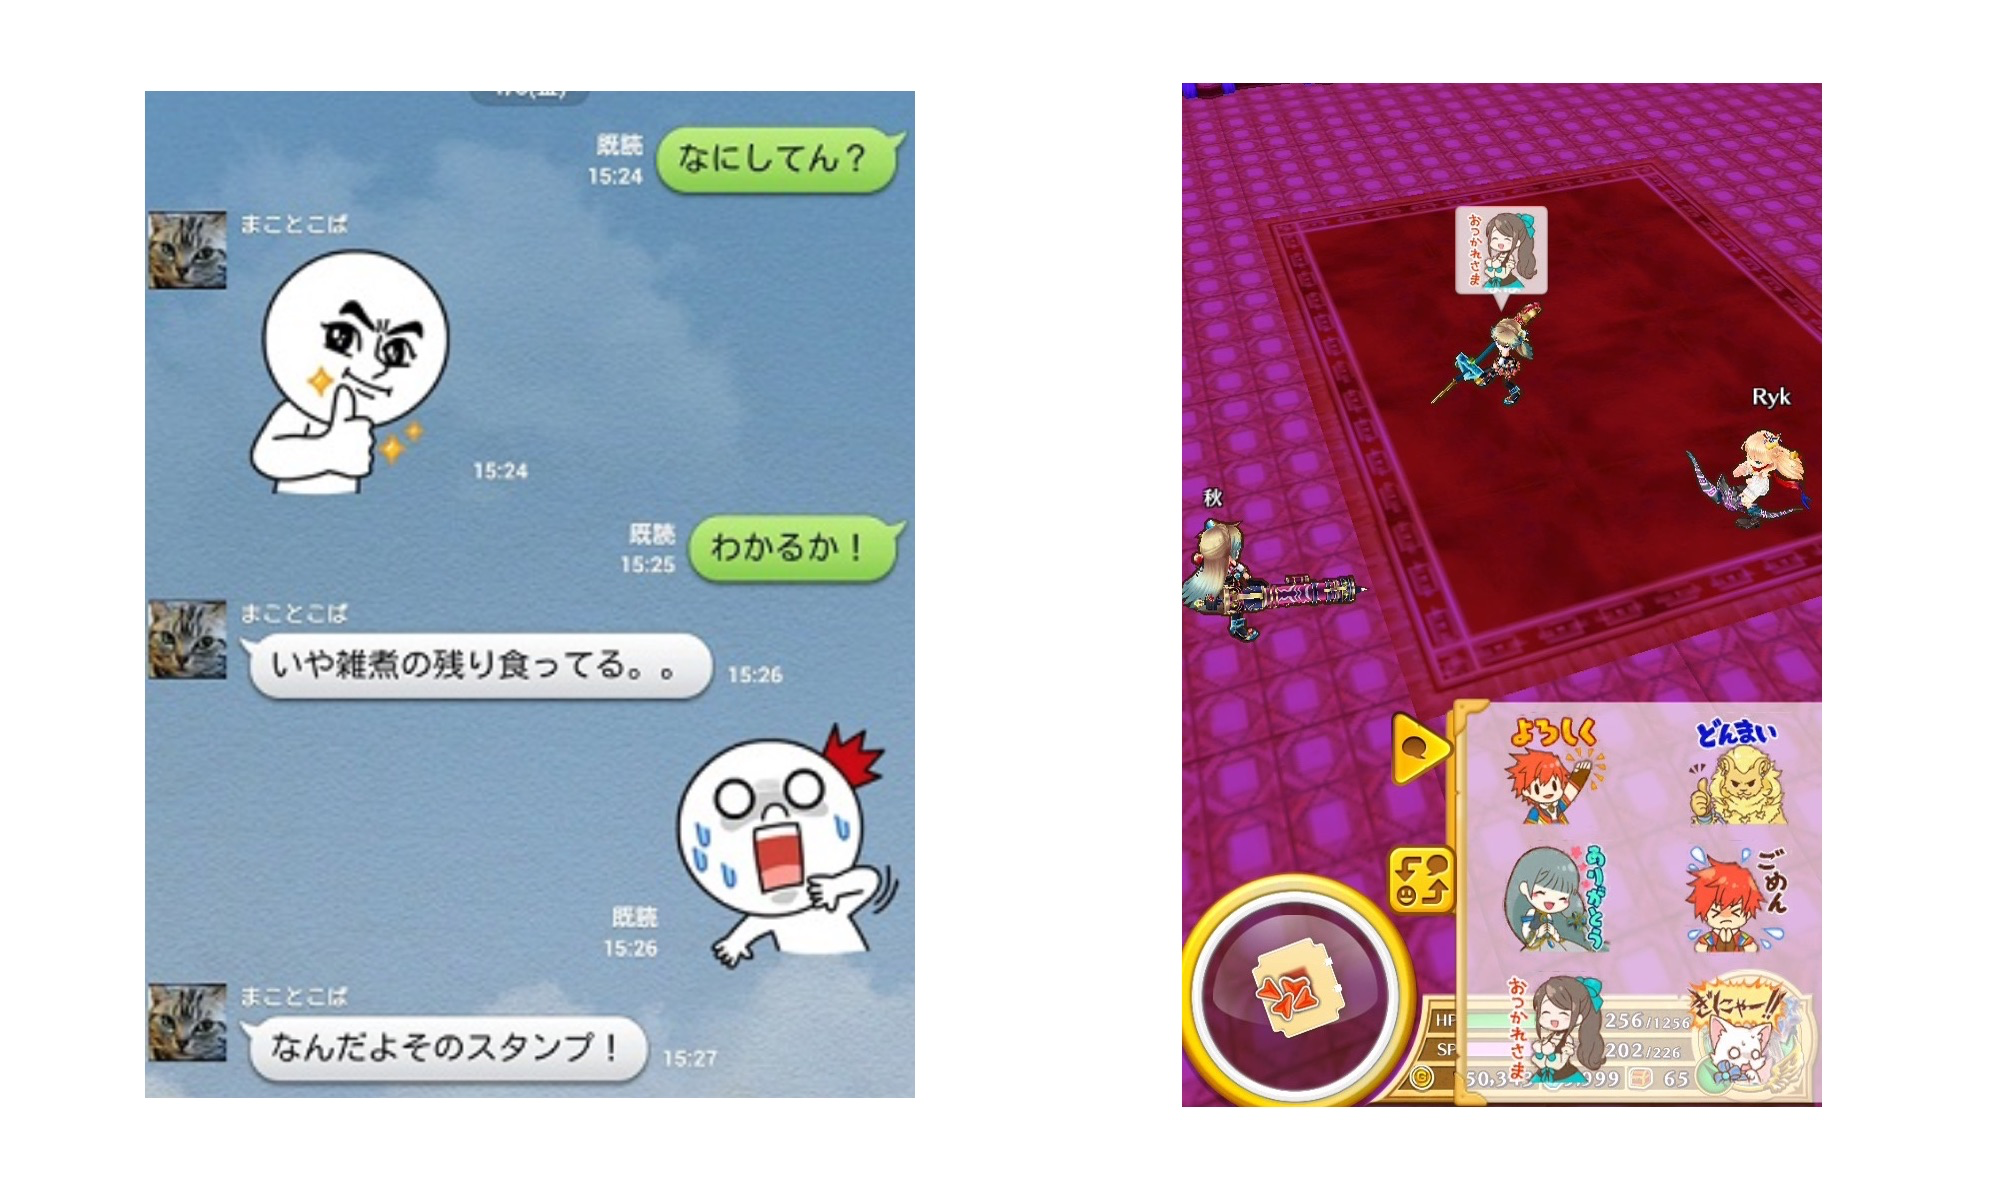
\includegraphics[width=11cm]{images/gamestamp.png}
\caption{LINEのトーク(左)とオンラインゲーム(右)で使われるスタンプ}
\label{gamestamp}
\end{figure}


\section{リアルタイムコンテンツ視聴中の情報共有}

発表や講演、テレビ放送などのリアルタイムコンテンツを視聴している際に、
他の視聴者はどのように感じたのか、知りたいことがある。
一人で視聴するよりも他の人と一緒に見た方が楽しかったり,
リビングで家族とテレビを見ながら団欒することが楽しかったりするのはそのためであり,
人と体験を共有することは重要なコミュニケーション手段である.

近年では、リアルタイムコンテンツを視聴中のコミュニケーションを行う様々なシステムが提供されている。
例えば、日本ソフトウェア科学会主催のWISS(Workshopn on Interactive Systems and Software)
コンファレンス\footnote{\textsf{http://wiss.org/}}では、
1997年から発表・聴講・議論・記録をサポートし盛り上げる新たなシステムを募集し、
会期中に実験的に運用されている\cite{wiss_challenge}。

動画投稿サイト「ニコニコ動画\footnote{http://www.nicovideo.jp}」では、
動画再生中にユーザがコメントをテキストを入力しボタンを押すことよって投稿され、投稿順に記録される。
記録されたコメントは他のユーザが同じ動画を鑑賞した場合にも反映され、
コメントが投稿された動画上のタイミングで動画上に重畳表示される(図\ref{niconico})。
コメントの投稿に時間差があっても、動画内の時間軸においては常に書き込まれた時と同じタイミングで表示されるため、
ユーザは実時間を超越した擬似的な時間共有を体感することが出来る。
これは、チャットや掲示板のような時系列に基づくメディアとは異なるユーザ体験をもたらしている\cite{110006793374}。

\begin{figure}[H]
\centering
\fbox{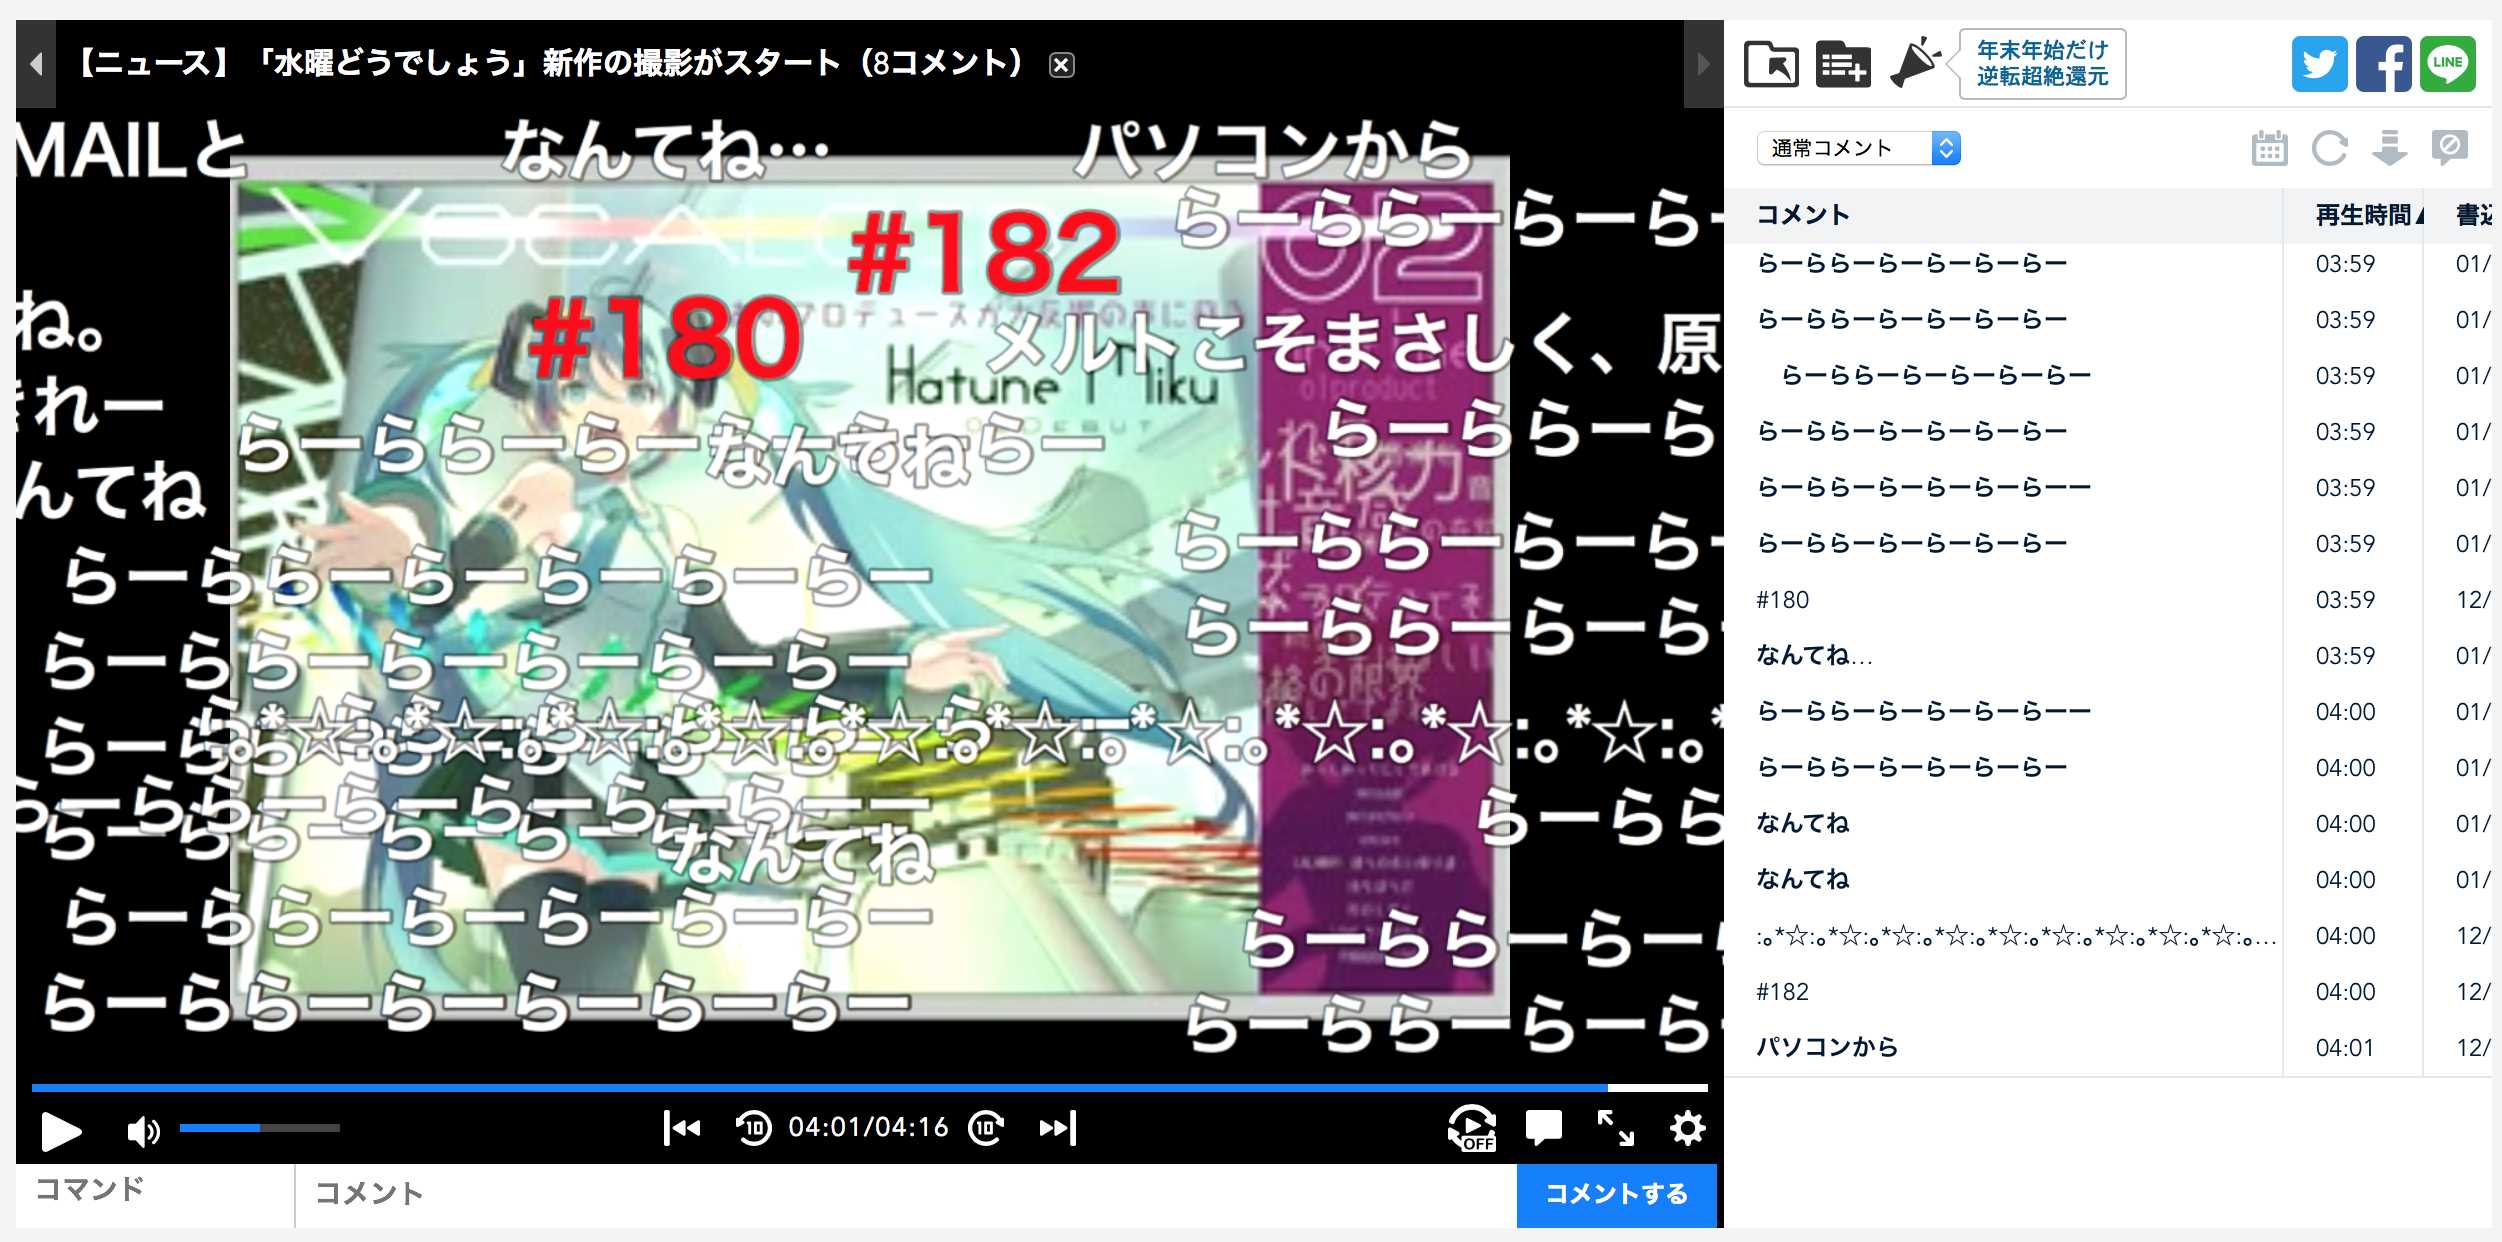
\includegraphics[width=10cm]{images/niconico.png}}
\caption{ニコニコ動画のコメント重畳表示}
\label{niconico}
\end{figure}


\section{情報ダッシュボード}

情報ダッシュボードは図\ref{azure}単一の画面に複数のリアルタイム情報を
タイル状に並べて表示するものである\cite{few}\cite{few2005}。
近年のICTやIoTなどの技術革新に伴い、センサーなどによる設備の稼動状況や
webから入手できる情報など大量の情報が溢れかえっている。
情報ダッシュボードはセンサの値や株価など常に値が変化していくものを複数並べて、
ひと目で把握するのに非常に便利なインタフェースである。
情報ダッシュボードには多くの製品やサービスが存在するが、
利用できる情報の種類は限られており、あらかじめ用意された種類の情報しか表示できない。

\begin{figure}[H]
\centering
\fbox{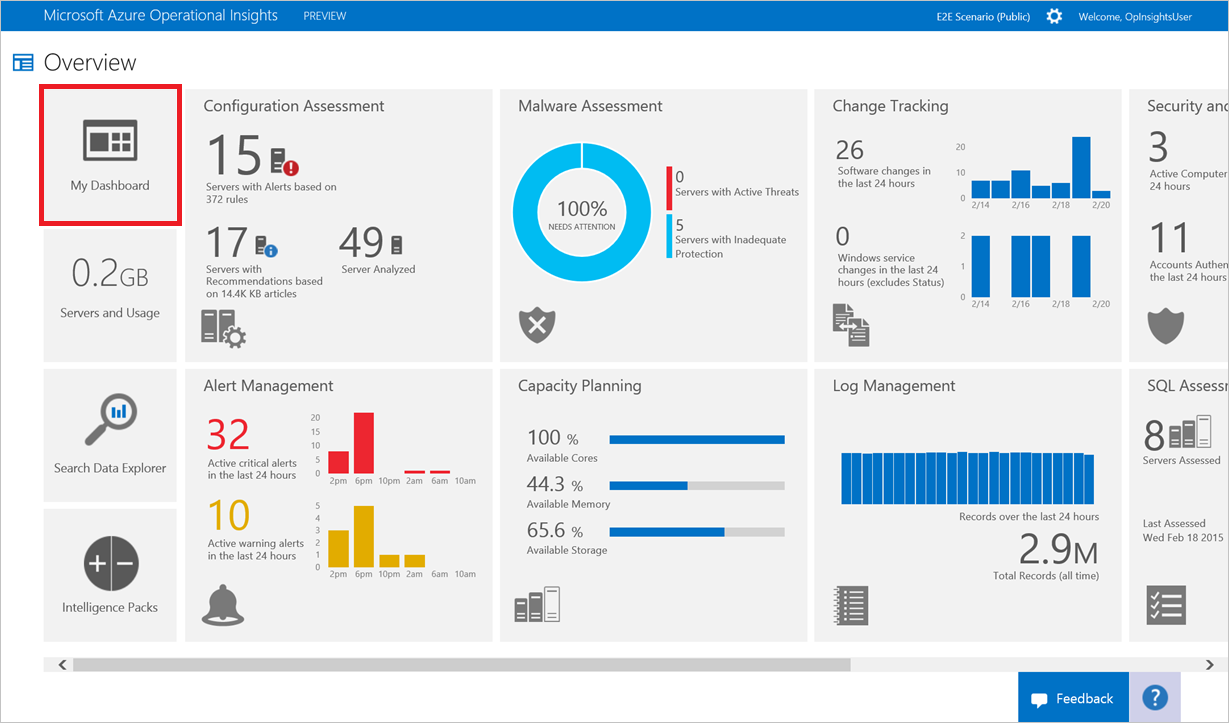
\includegraphics[width=10cm]{images/azure.png}}
\caption{Microsoft Azureの情報ダッシュボード}
\label{azure}
\end{figure}